\author{Florian Müller}
\graphicspath{ {./src/chapters/developer/media/ld_live/} }
\section {opencv}

opencv can be installed via pip and used via \texttt{import cv2}.
For the scripts here, the \texttt{opencv-contrib-python} package was loaded and imported as cv.

All examples are thus called only with cv and not with cv2.

\subsection {Blur}

\texttt{image = cv.blur(img, kernel)}

The function \texttt{blur()} is used to soften an image.
A kernel is applied to each pixel in the image and computed.

This kernel is a normalized matrix filled with ones.
As an example a 3x3 normalized matrix can be considered here:

$$Kernel = \frac{1}{9}
\begin{bmatrix}
1 &1 &1 \\
1 &1 &1 \\
1 &1 &1
\end{bmatrix}
$$


\subsection {Dilate and Erode}

\texttt{kernal = cv.getStructuringElement(cv.MORPH\_ELLIPSE, (x-size, y-size))}

\texttt{dilated\_image = cv.dilate(image, kernel)}

\texttt{eroded\_image = cv.erode(image, kernel)}

Dilation and erosion are very similar to describe.
In both operations an image $A$ will be convolved with a kernel $B$.
The usage of both functions are removing noise, isolate individual elements, closing gaps in images.

The dilation or grow function is used to let an image grow in the directions of the kernel.
But it is also possible to set the anchor of the kernal not to the centre but to a different point.
Then it is possible to let the picture grow or shrink in a specific direction.
e.g.:

\texttt{cv.dilate(image, kernel, anchor = (1,1))}

For the erosion the same kernel can be used.
And instead of letting the image grow, with an erosion the image will shrink.
This can be used to eliminate noise or separate elements which are barely touching.

The function itself is passed two parameters and then returns a modified image.

The opencv docs contain a good explanation\\
\url{https://docs.opencv.org/3.4/db/df6/tutorial\_erosion\_dilatation.html}

\subsection{Convert Color}

\texttt{image = cv.cvtColor(image, flag)}

During the color conversion the function receive two arguments and returns the converted picture.
The first argument is the image to convert.
The second argument is the flag which conversion shall be used.
For this project only the \texttt{BGR2GRAY} and \texttt{RGB2BGR} flags are used.

\subsection{Threshold}

\texttt{threshold, image = cv.threshold(image, min, max, flag)}

Threshold is used to remove some noise and to convert the image to a binary format.
This function receive four arguments and returns two outputs.
The first output is the used threshold and the second is the thresholded picture.

The first input is the image to be thresholded, which should be already converted to grayscale.
\texttt{min} is the actual threshold which determines if a pixel is set to zero or to the \texttt{max} value.
The flags will determine which threshold algorithm will be used.
The two mainly used flags are \texttt{cv.THRESH\_OTSU} and \texttt{cv.THRESH\_BINARY\_INV}.

\texttt{cv.THRESH\_BINARY\_INV} is the simpler one of both.
After calculating the threshold for each pixel the resulting image will be inverted.
This kind of image can be used for further processing.

\texttt{cv.THRESH\_OTSU} is a more complex algorithm.
During the thresholding process the \texttt{min} value will be calculated automatically.
The \texttt{cv.THRESH\_OTSU} flag has to be set as an extra flag to the already given flag.
Now the \texttt{min} value will be substitued by the Otsu's calculated value.

\subsection{Find Contours}

\texttt{contours, hirachy = cv.findContours(image, return\_flag, approximation\_flag)}

A contour can be understood as a curve joining all pixels of the same value like color or intensity.
The function receives three arguments and returns two outputs.
For the outputs the first is a list with points for the contours.
The second one is a list with the same length as the first one with values determing the neighbours and the depth of the contour.

The fist argument is the image in with the contours will be searched.
For best computing time it is recommended to use a grayscale or binary image.
The second argument determine which kind of list of contours will be returned.
The three recommended flags are \texttt{cv.RETR\_LIST}, \texttt{cv.RETR\_TREE} and \texttt{cv.RETR\_EXTERNAL}.
For this project the \texttt{cv.RETR\_EXTERNAL} flag is the mostly used.
With this flag only the top level contours will be returned without inner contours.
The third argument determines how many points will be used for the contour.
The flag \texttt{cv.CHAIN\_APPROX\_NONE} is the commonly used to detect all points of a contour.
This makes it possible to draw a perfect mask for each found symbol.
% TODO an example would be nice

\begin{figure}[H]
    \centering
    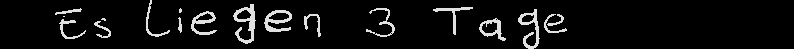
\includegraphics[width=.8\textwidth]{line10000.png}
    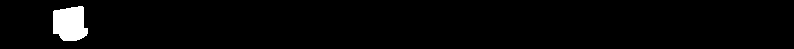
\includegraphics[width=.8\textwidth]{mask10005.png}
    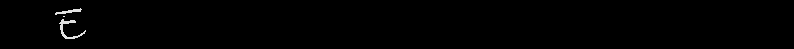
\includegraphics[width=.8\textwidth]{01result.png}
    \caption{Example for masking one letter}
\end{figure}

\subsection{Bounding Rectangle}

\texttt{x, y, w, h = cv.boundingRect(contour)}

For each contour this function will output the bounding rectangle.
It is possible to draw the rectangle or cut the area.
For letterdetection this is used to cut out the individual charakters after the masking process.

\subsection{arcLength and approxPolyDP}

\texttt{epsilon = value * cv.arcLength(contour, bool)}

\texttt{approximation = cv.approxPolyDP(contour, epsilon, bool)}

These functions are used to approximate a contour which isn't in a perfect shape.
For example a square which isn't detected correctly can be found with this approximation.
The \texttt{cv.arcLength()} function returns the length of a contour.
The bool values dertermine if the contour is closed or just a curve.
The \texttt{cv.approxPolyDP()} function is an implementation of the Ramer-Douglas-Peucker algorithm.
In a nutshell it will calculate a contour with lesser points than the original given contour.
For more information about this algorithm please visit \url{https://en.wikipedia.org/wiki/Ramer\_Douglas\_Peucker\_algorithm}.

